\subsection{Estado del Arte}

\subsubsection{Migración de plataformas Firebase hacia arquitecturas en AWS}

Como lo indica J. Michel \cite{Michael2021}, Firebase ofrece una arquitectura de dos capas, donde las aplicaciones cliente (web o móviles) interactúan directamente con servicios \textit{backend} como Firestore, Authentication y Cloud Functions. Esta simplicidad facilita el desarrollo rápido de MVPs, pero puede presentar desafíos en escalabilidad, control y flexibilidad a medida que la aplicación crece. Obsérvese la \autoref{fig:firebase_architecture}.

\newcommand\firebaseArchitectureCaption{Diagrama de Arquitectura de Firebase. \hspace{1em}}

\begin{figure}[H]
  \centering
  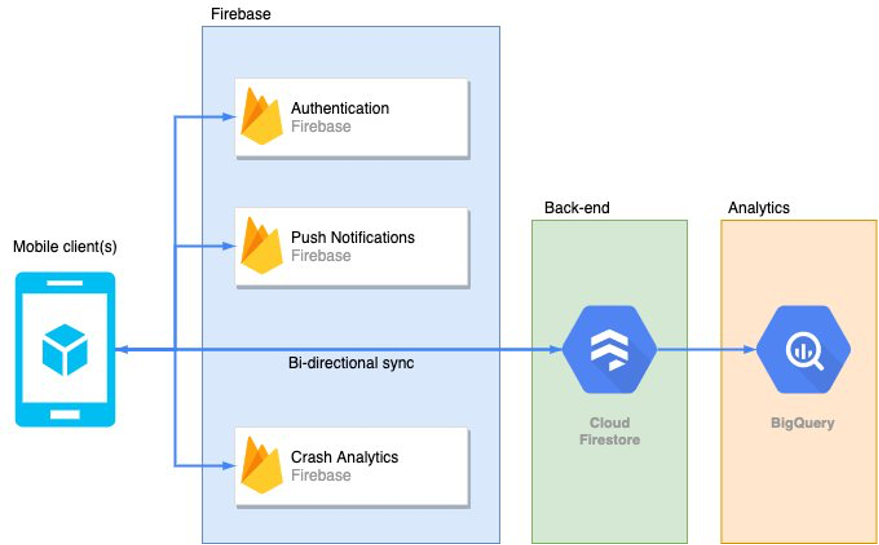
\includegraphics[width=0.7\textwidth]{img/figures/fig3-firebase-architecture.png}
  \caption[\firebaseArchitectureCaption]{\firebaseArchitectureCaption Fuente: Tomado de \cite{Michael2021}.}
  \label{fig:firebase_architecture}
\end{figure}

En contraste, como se muestra en la \autoref{fig:amplify_architecture}, AWS adopta una arquitectura de tres capas, donde se separan de forma clara la capa de presentación, la lógica de negocio y la capa de datos. Esta organización modular permite un mayor control, escalabilidad y mantenibilidad del sistema, además de reducir significativamente el riesgo de exponer lógica de negocio crítica en el cliente.

En este enfoque, el cliente utiliza el SDK de AWS Amplify para comunicarse con los servicios del \textit{backend}, los cuales están implementados mediante funciones Lambda, las cuales pueden ser accedidas mediante una API REST usando Amazon API Gateway. De esta forma, se evita el acceso directo desde el frontend a las bases de datos o a la lógica sensible del negocio, incrementando la seguridad y permitiendo una evolución más controlada de la arquitectura.

\newcommand\AWSDiagramaArquitecturaCaption{Diagrama de Arquitectura de AWS Amplify. \hspace{1em}}

\begin{figure}[H]
  \centering
  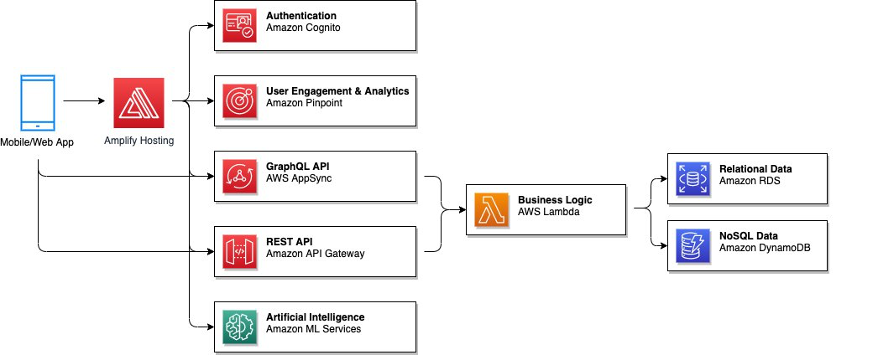
\includegraphics[width=1\textwidth]{img/figures/fig4-amplify-architecture.png}
  \caption[\AWSDiagramaArquitecturaCaption]{\AWSDiagramaArquitecturaCaption Fuente: Tomado de \cite{Michael2021}}
  \label{fig:amplify_architecture}
\end{figure}

A diferencia de Firebase, donde todos los servicios están integrados dentro de una misma plataforma, AWS ofrece un enfoque más flexible y modular. Herramientas como AWS Amplify y el Amazon Cloud Development Kit (CDK) permiten definir, configurar e implementar servicios \textit{backend} de forma personalizada \cite{Michael2021}. Amplify proporciona un conjunto de herramientas para el desarrollo, incluyendo SDKs, generación automática de código y una pipeline DevOps que facilita la integración entre los servicios de AWS y las aplicaciones web o móviles \cite{Michael2021}.

Este enfoque permite construir arquitecturas completamente adaptadas a las necesidades del proyecto, seleccionando únicamente los servicios requeridos. Además, gracias al uso de Infraestructura como Código (IaC) mediante CDK o CloudFormation, es posible versionar, reutilizar y automatizar la configuración de los recursos, mejorando la mantenibilidad y escalabilidad del sistema.

Por otro lado, la migración de Firebase a AWS implica identificar servicios equivalentes que ofrezcan funcionalidades similares, pero con mayor flexibilidad y escalabilidad. La \autoref{tab:aws_firebase_comparison_services} presenta la correspondencia general entre servicios de Firebase y sus equivalentes en AWS.

\newcommand\correspondenciaFirebaseAWSCaption{Correspondencia general entre los servicios de Firebase y sus equivalentes en AWS. \hspace{1em}}
\begin{table}[H]
  \centering
  \begin{tabular}{|l|l|}
    \hline
    \grayTableHeaderCell{6cm}{Funcionalidad Firebase} & \grayTableHeaderCell{8cm}{Servicio AWS Equivalente} \\

    \hline
    Firebase Authentication & Amazon Cognito \\
    \hline
    Cloud Firestore & Amazon DynamoDB \\
    \hline
    Firebase Cloud Functions & AWS Lambda \\
    \hline
    Firebase Cloud Messaging & Amazon SNS \\
    \hline
    Cloud Storage & Amazon S3 + Amazon CloudFront \\
    \hline
    Firebase Hosting & AWS Amplify \\
    \hline
  \end{tabular}
  \caption[\correspondenciaFirebaseAWSCaption]{\correspondenciaFirebaseAWSCaption Fuente: Elaboración propia.}
  \label{tab:aws_firebase_comparison_services}
\end{table}

Esta correspondencia permite a las aplicaciones migradas beneficiarse de la robustez y escalabilidad de los servicios de AWS, adaptándose mejor a las necesidades empresariales en crecimiento.

Actualmente, la plataforma de Paralegales utiliza únicamente algunos servicios clave de Firebase: Firebase Authentication para la gestión de usuarios, Cloud Firestore como base de datos NoSQL y lógica de negocio crítica implementada directamente en el cliente. Esta última representa un riesgo de seguridad, ya que expone operaciones sensibles en el frontend. Como parte del proceso de migración a AWS, estos componentes serán reemplazados por servicios equivalentes más robustos y seguros: Amazon Cognito asumirá la autenticación de usuarios, Amazon DynamoDB gestionará los datos, y la lógica de negocio crítica será trasladada a funciones AWS Lambda, ejecutadas desde el \textit{backend}.

La migración de una plataforma desde Firebase a AWS requiere una planificación cuidadosa para minimizar interrupciones, preservar la integridad de los datos y garantizar una experiencia fluida para los usuarios. En el caso de Paralegales, esta transición está prevista una vez que la aplicación esté en producción y cuente con usuarios reales, lo que hace aún más crucial la implementación de estrategias que permitan una migración progresiva y controlada. A continuación, se describen las principales estrategias consideradas para llevar a cabo este proceso.

\subsubsection{Migración de usuarios de Firebase a Amazon Cognito}

Como lo indica A. Hall en el blog de AWS \cite{Hall2017}, Existen dos métodos principales para migrar usuarios:

\begin{enumerate}[label=\alph*)]

\item \textbf{\textit{Importación por lotes}}: Consiste en exportar los datos de usuario desde Firebase y cargarlos en Amazon Cognito mediante un archivo CSV. Es importante destacar que las contraseñas no se migran, por lo que los usuarios deberán restablecerse al iniciar sesión por primera vez en el nuevo sistema.

\item \textbf{\textit{Migración individual al iniciar sesión}}: Esta estrategia permite migrar usuarios a medida que inician sesión. Si un usuario no existe en Cognito, se autentica mediante Firebase y luego se crea su cuenta en Cognito, permitiendo una transición sin interrupciones para el usuario.
\end{enumerate}

\subsubsection{Migración de datos de Firestore a DynamoDB}

La migración de datos puede realizarse mediante los siguientes enfoques complementarios:

\begin{enumerate}[label=\alph*)]
\item \textbf{\textit{Carga Masiva}}: La migración de datos desde Cloud Firestore hacia Amazon DynamoDB requiere más que una simple operación de exportación e importación, ya que los modelos de datos de ambas bases de datos no son completamente compatibles. Por ello, se recomienda implementar una pipeline de tipo ETL (\textit{Extract, Transform, Load}) que permita transformar y adaptar los datos durante el proceso de migración \cite{Michael2021}.

\hfill

Esta pipeline puede construirse utilizando servicios totalmente gestionados de AWS, como AWS Step Functions para la orquestación del flujo, AWS Lambda para ejecutar cada una de las etapas del proceso de extracción, transformación y carga, y Amazon SQS para manejar la comunicación entre pasos mediante colas de mensajes. Este enfoque garantiza durabilidad y capacidad de re-ejecución de los trabajos en caso de fallos, a la vez que minimiza la carga operativa y reduce los costos al utilizar servicios \textit{serverless} \cite{Michael2021}.

\item \textbf{\textit{Sincronización en Paralelo}}: Durante un período de transición, operar ambas bases de datos en paralelo, sincronizando los cambios en tiempo real para garantizar la consistencia de los datos hasta completar la migración.
\end{enumerate}

\subsubsection{Referencia práctica de migración: implementación basada en AWS CDK}

Además de la documentación oficial, B. Shank \cite{Shank2021}, Sr. Startup SA en AWS, implementó un repositorio de código abierto en en AWS CDK que puede servir como guía práctica para realizar la migración. Dicho repositorio, incluye dos fases de despliegue y múltiples \textit{stacks} que replican los servicios clave de Firebase: Firestore, Authentication y Cloud Storage, utilizando sus equivalentes en AWS (DynamoDB, Cognito y S3, respectivamente).

\newcommand\DiagramaMigracionAWSCaption{Diagrama de Infraestructura de la migración propuesta por B. Shank. \hspace{1em}}
\begin{figure}[H]
\centering
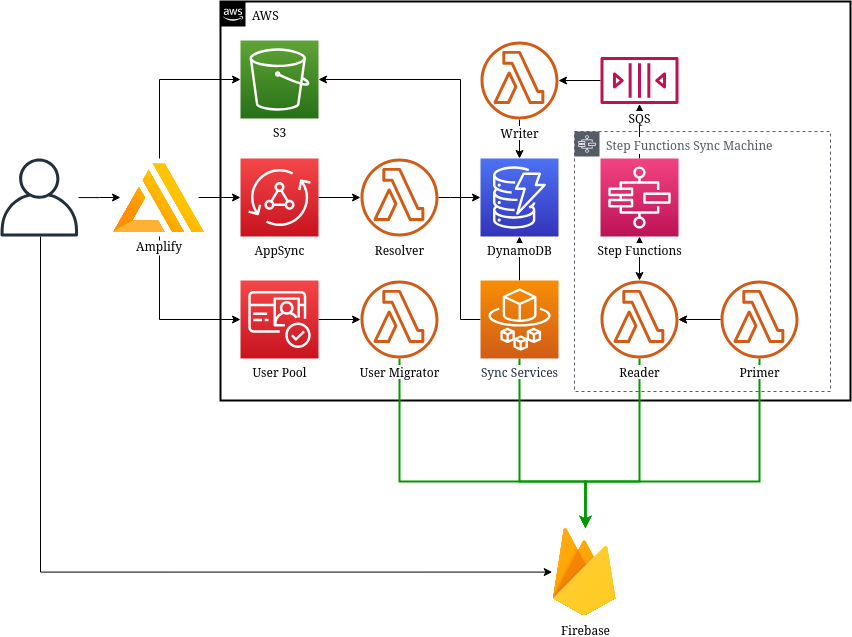
\includegraphics[width=0.9\textwidth]{img/figures/fig5-etl-pipeline-aws.png}
\caption[\DiagramaMigracionAWSCaption]{\DiagramaMigracionAWSCaption Fuente: Tomado de \cite{Shank2021}.}
\label{fig:aws_migration_pipeline}
\end{figure}

En la primera fase ilustrada en la \autoref{fig:aws_migration_pipeline}, se aprovisionan los recursos base y se ejecuta automáticamente una máquina de estados de AWS Step Functions que extrae y transforma los datos desde Firestore para cargarlos en DynamoDB, utilizando un esquema de tabla única. En paralelo, los usuarios de Firebase Authentication se migran a Amazon Cognito a través de un trigger Lambda específico durante el despliegue.

La segunda, también detallada en la \autoref{fig:aws_migration_pipeline}, fase despliega una API GraphQL con AppSync, cuya definición se genera automáticamente a partir de los datos sincronizados. También incluye un servicio en AWS Fargate que escucha eventos en tiempo real desde Firestore y sincroniza los cambios con DynamoDB. Esta arquitectura híbrida permite mantener ambas plataformas operando en paralelo durante el proceso de transición, lo que resulta especialmente útil para reducir el riesgo al migrar una aplicación en producción.

\subsubsection{Bibliografía Complementaria}
Como complemento a los enfoques técnicos revisados, el trabajo de \textcite{Kansara2024} aporta una visión más amplia sobre los desafíos y metodologías emergentes en procesos de migración de bases de datos hacia la nube. Su estudio enfatiza la automatización, la integridad de los datos y la optimización del rendimiento como pilares fundamentales para garantizar migraciones eficientes y seguras. En particular, el autor presenta un diagrama de alto nivel que descompone el proceso en fases estructuradas: extracción y validación de datos, refactorización de lógica de negocio, transferencia segura y orquestación de servicios en la nube. Esta representación, ilustrada en la \autoref{fig:etl_process_diagram}, proporciona un marco útil para entender la transición desde arquitecturas legadas hacia entornos escalables y distribuidos basados en servicios nativos de la nube.

\newcommand\migrationProcessDiagramCaption{Diagrama del proceso de migración a base de datos en la nube. \hspace{1em}}
\begin{figure}[H]
\centering
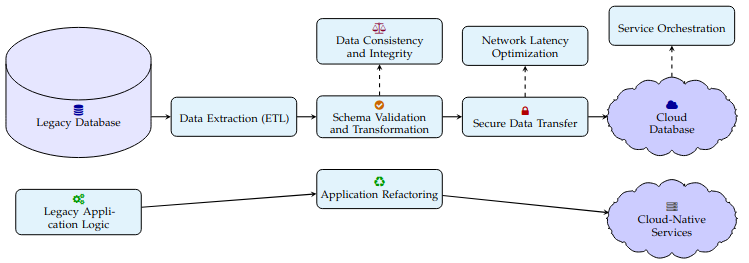
\includegraphics[width=1\textwidth]{img/figures/fig6-etl-process.png}
\caption[\migrationProcessDiagramCaption]{\migrationProcessDiagramCaption Fuente: Tomado de \cite{Kansara2024}.}
\label{fig:etl_process_diagram}
\end{figure}

Por otro lado, en la literatura complementaria se encuentra el trabajo de \textcite{Kyadasu2025}, quienes, a través de un estudio de caso sobre migración entre proveedores de nube, explican cómo las prácticas DevOps, con su enfoque en la automatización y la integración y entrega continuas (CI/CD), ofrecen beneficios significativos y presentan lo que consideran como mejores prácticas para llevar a cabo este tipo de procesos.
